\documentclass[usepdftitle=true]{beamer}
\usetheme{Madrid}
\usepackage[utf8]{inputenc}
\usefonttheme{professionalfonts}
\usepackage{graphicx}

\author{Filip Cima}
\title{Alternative Sources of Energy}
\institute{VŠB - TUO}

\begin{document}

\frame{\titlepage}

\begin{frame}[<+->]
	\frametitle{What will we learn?}
	Existing types of alternative energy:
	\begin{itemize}[<+->]
		\item Solar energy	
		\item Wind energy
	 	\item Hydroelectricity
		\item Geothermal energy
		\item Biomass
	\end{itemize}
	How could a community be self-sufficient in energy?
	\begin{itemize}
		\item Is it possible?
		\item When?
	\end{itemize}
\end{frame}

\begin{frame}
	\frametitle{Alternative sources of energy}
	\begin{itemize}[<+->]
		\item Alternative energy is any energy source that is an alternative to fossil fuel.
		\item They are natural resources that are partially or completely renewed when consuming gradually.
	\end{itemize}
	\begin{figure}
		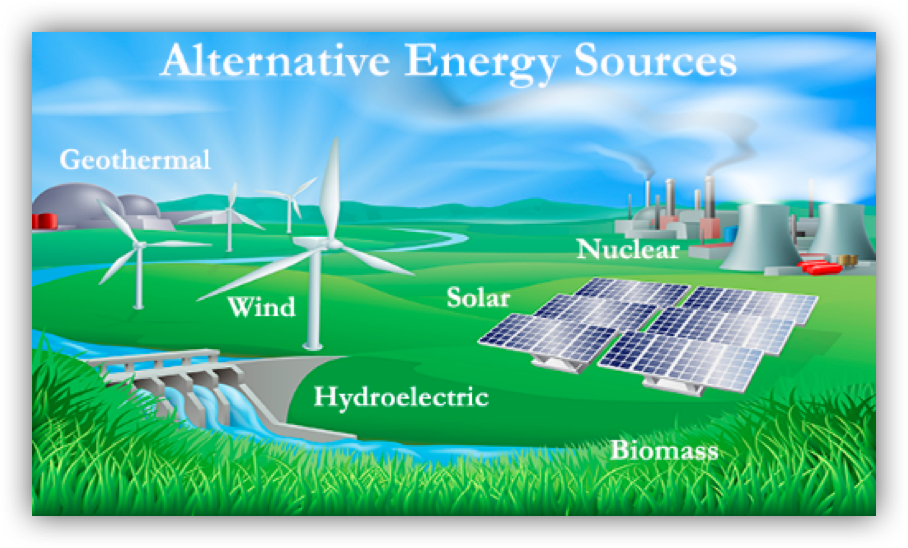
\includegraphics[scale=0.38]{img/typesofenergy.png}
	\caption{Most known types of energy}
	\end{figure}
\end{frame}

\begin{frame}
	\frametitle{Solar energy}
	\begin{columns}
		\column{0.65\textwidth}
			Solar energy can be used for heating, cooling or electrical power generation using the sun.
			\textbf{Solar powerplant:}
			\begin{itemize}
				\item Uses photovoltaic panels (made of silicon, the conversion of light into electricity)
				\item When the sun rays fall on the panels, electrons are released which is involved in the generation of electric current.
			\end{itemize}
			\textbf{Advantages:}
			\begin{itemize}
				\item Easy to use 
			\end{itemize}
			\textbf{Disadvantages:}
			\begin{itemize}
				\item High initial costs
				\item Solar fluctuations
			\end{itemize}
		\column{0.35\textwidth}
			\begin{figure}
				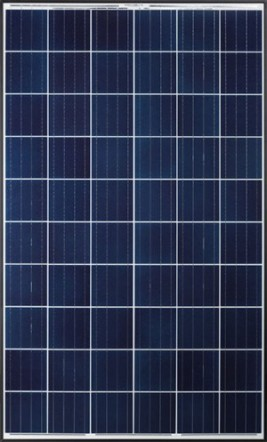
\includegraphics[scale=0.40]{img/solar_panel_flat.jpg}
				\caption{Solar panel}
			\end{figure}
	\end{columns}
\end{frame}

\begin{frame}
	\frametitle{Wind power plant}
	Wind power plants uses \textbf{wind flow} as a source of energy.
	They are mostly used in \textbf{Spain, Germany and Denmark, Netherland and Austria}.
	Electricity production in the Czech Republic is around 1 \%.
	\vspace{0.25cm}
	\newline
	\textbf{Advantages:}
	\begin{itemize}
		\item Without emissions
		\item Without waste
		\item Without burdening the land
	\end{itemize}
	\textbf{Disadvantages:}
	\begin{itemize}
		\item Variability of wind power
		\item Noisy
		\item Complex location
	\end{itemize}
\end{frame}

\begin{frame}
	\frametitle{Wind power plant}
	\textbf{How it works?}
	\begin{itemize}
		\item Turbines are on towers (50-80 metres)
		\item Electromagnetic induction
	\end{itemize}
	\center
	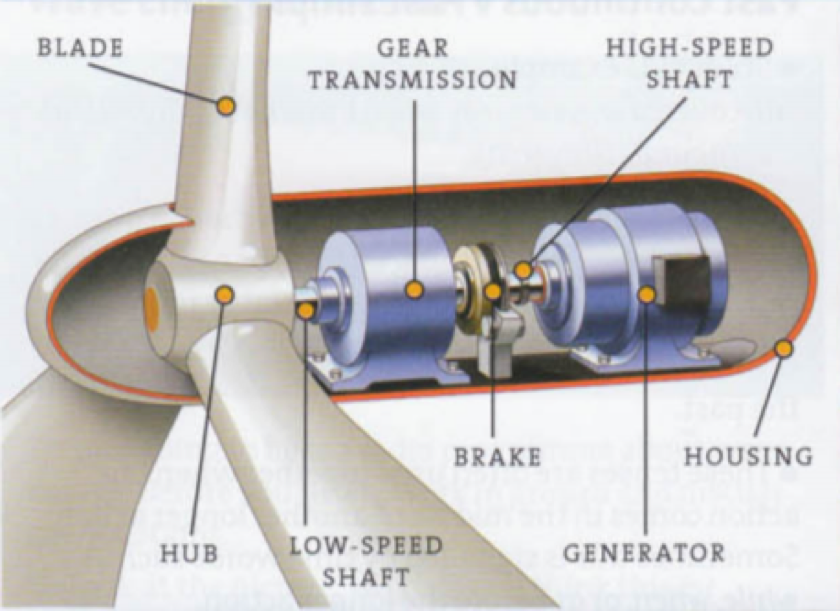
\includegraphics[scale=0.40]{img/wind_turbine.png}
\end{frame}

\begin{frame}
	\frametitle{Biomass}
	Is organic matter (wood, straw, …) 
	Energy is obtained through the combustion (burning) process\newline
	Electricity production in the Czech Republic is around 2,8 \%
	\vspace{0.25cm}
	\newline
	\textbf{Advantages:}
	\begin{itemize}
		\item Low CO\textsubscript{2} emissions
		\item Availability
	\end{itemize}
	\textbf{Disadvantages:}
	\begin{itemize}
		\item Low efficiency
		\item Storage space
	\end{itemize}
\end{frame}

\begin{frame}
	\frametitle{Hydroelectric power station}
	The flowing water rotates the turbine, the generator converts mechanical energy into electrical energy and transforms it into places of need.
	\center
	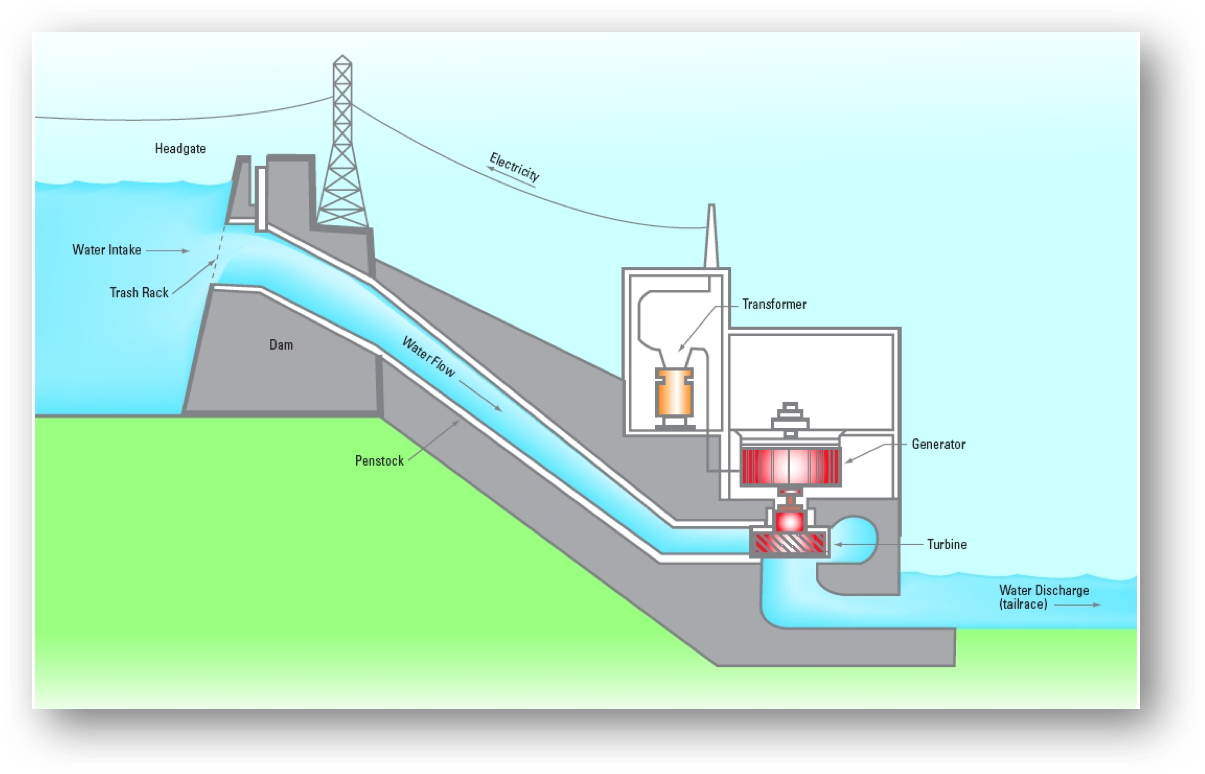
\includegraphics[scale=0.45]{img/water_plant.png}
\end{frame}

\begin{frame}
	\frametitle{Geothermal energy}
	\textbf{Geothermal power plant}
	\begin{columns}
		\column{0.5\textwidth}
			\begin{itemize}
				\item It produces electricity from heat from the Earth (hot steam, springs).
				\item Construction in volcanically active areas.
				\item \textbf{Iceland}, Italy, \textbf{New Zealand}
			\end{itemize}
		\column{0.5\textwidth}
			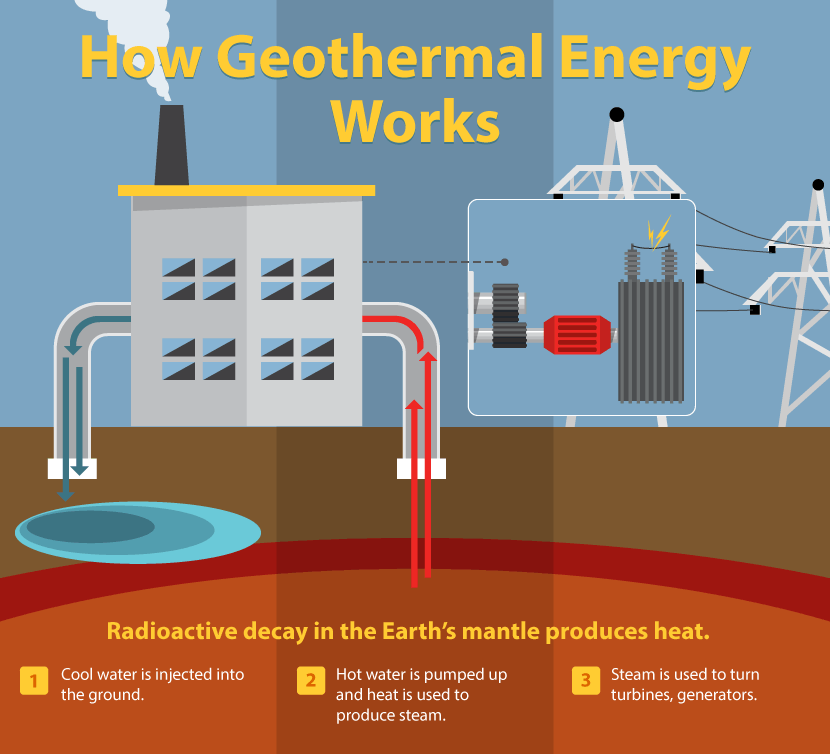
\includegraphics[scale=0.2]{img/geothermal-energy.png}
	\end{columns}
\end{frame}

\begin{frame}
	\frametitle{Self sufficient community?}
	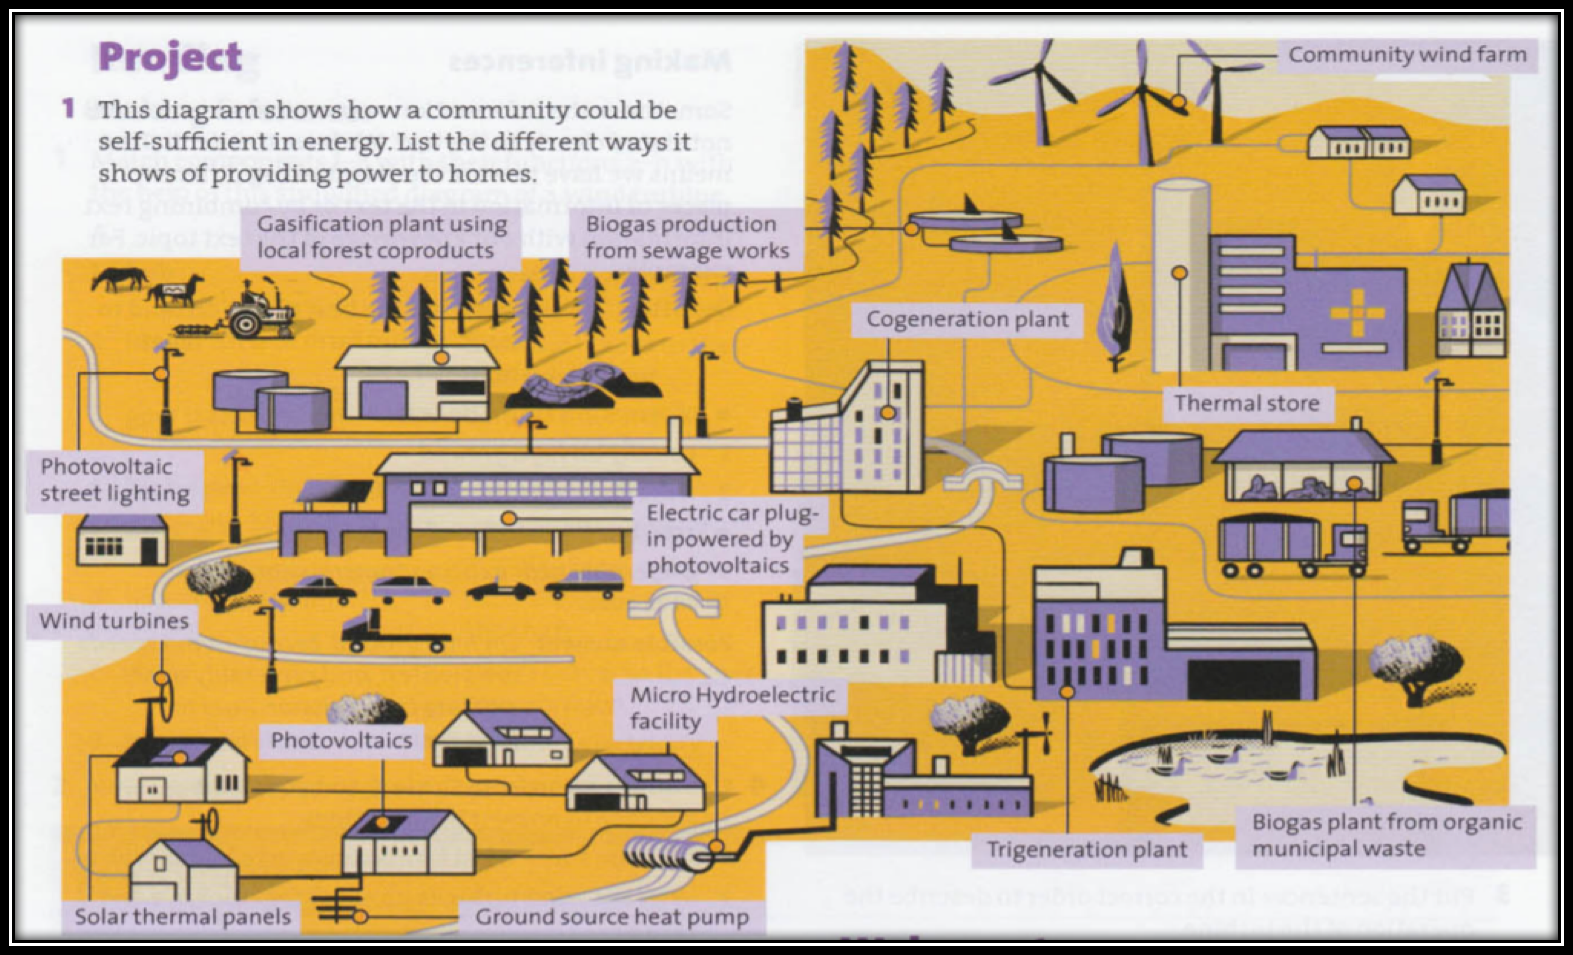
\includegraphics[scale=0.45]{img/textbook.png}
\end{frame}

\begin{frame}
	\centering \Huge \emph{Thank you for your attention!}
\end{frame}

\end{document}	